\documentclass{article}
%
% Demo of the mcode package from 
% http://www.mathworks.co.uk/matlabcentral/fileexchange/8015-m-code-latex-package
% Updated 06 Mar 2014
%

\usepackage{graphicx}
\usepackage{wrapfig}
\usepackage{mathtools}
\usepackage{mathrsfs}
\usepackage{enumitem}
\usepackage{pdflscape}
\graphicspath{ {images/} }

% load package with ``framed'' and ``numbered'' option.
\usepackage[framed,numbered,autolinebreaks,useliterate]{mcode}

% something NOT relevant to the usage of the package.
\usepackage{url}
\setlength{\parindent}{0pt}
\setlength{\parskip}{18pt}


% //////////////////////////////////////////////////

\begin{document}

\title{Homework 1 - Optimal Control Systems}
\author{Erivelton Gualter dos Santos, 2703806}
\date{}

\maketitle 

\begin{wrapfigure}{l}{0.3\textwidth}
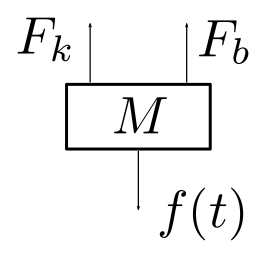
\includegraphics [width=1in]{output}
\caption{Free-Body Diagram for Exercise 1.3 - Kirk.}
\end{wrapfigure} 

\begin{enumerate}[label=(\alph*)]
\item State equations for the mechanical system show in Fig. 1-P3 at Kirk.
\end{enumerate}

The following figure describes the free-body diagram. The governing equation for this system is:

\begin{equation*}
\ddot{y} = \frac{f - Ky - B\dot{y}}{M}
\end{equation*}

Defining the \textit{States Variables} $x_1$ and $x_2$ as $y$ and $\dot{y}$ respectively, we have: 
\begin{eqnarray}\label{i1}
\begin{split}
	\dot{x_1} &= x_2 \\
	\dot{x_2} &= -\frac{K}{M}x_1 -\frac{B}{M}x_2 +\frac{1}{M}f
\end{split}
\end{eqnarray}

Also, these differential equations can be written as the following matrix notation:
\begin{eqnarray*}
\begin{bmatrix} 
	\dot{x_1} \\ 
	\dot{x_2} \\
\end{bmatrix} &= 
\begin{bmatrix} 
    0  &   1 \\
    -\frac{K}{M}  &  -\frac{B}{M} \\
\end{bmatrix} 
\begin{bmatrix}
	x_1 \\
	x_2 
\end{bmatrix} +
\begin{bmatrix}
	0 \\ \frac{1}{M}
\end{bmatrix}f 
\end{eqnarray*}
 
\begin{enumerate}[label=(\alpha*)]
\item[(c)] Determine the state transition matrix $\varphi(t)$.
\end{enumerate}

Assuming that $M = 1\:kg$, $K = 2\:\frac{N}{m}$ and $B = 2\:\frac{N}{m/s}$, we have:
\begin{eqnarray*}
\begin{bmatrix} 
	\dot{x_1} \\ 
	\dot{x_2} \\
\end{bmatrix} &= 
\begin{bmatrix} 
    0  &   1 \\
    -2  &  -2\\
\end{bmatrix} 
\begin{bmatrix}
	x_1 \\
	x_2 
\end{bmatrix} +
\begin{bmatrix}
	0 \\ 1
\end{bmatrix}f \\
\end{eqnarray*}

The solution for the state equations in \ref{i1} is:
\begin{equation}
x(t) = \varphi(t,t_0)x(t_o) + \int_{t_o}^{t} \varphi(t,\tau)B(\tau)u(\tau) d\tau
\end{equation}
where, $\varphi(t,t_0)$ is the \textit{state transition matrix}. For a LTI system, it also ca be given as:
\begin{equation}
x(t) = \mathcal{L}^{-1} \left\lbrace \left[sI-A \right]^{-1}x(0) + \left[sI-A \right]^{-1}BU(s) \right\rbrace
\end{equation}\label{xt}
where, the \textit{State Transition Equation} correspond to $ \left[sI-A \right]^{-1} $. Therefore, 
\begin{eqnarray*}
\varPhi(s) =
\begin{bmatrix} 
sI-A
\end{bmatrix}^{-1} = 
\begin{bmatrix} 
    s  &   -1 \\
    2  &  s+2\\
\end{bmatrix} ^{-1} = \frac{1}{s^2+ 2s+ 2}
\begin{bmatrix}
    s+2 & 1	\\
    -2  & s \\
\end{bmatrix}
\end{eqnarray*}
According to the Laplace Table \ref{laplace}, 
\begin{table}[h]
\centering
\caption{Table of Laplace Transforms}
\label{laplace}
\begin{tabular}{|l|l|}
\hline
$e^{at}\sin kt$ & $\dfrac{k}{(s-a)^2+k^2}$  \\ \hline
$e^{at}\cos kt$ & $\dfrac{s-a}{(s-a)^2+k^2}$ \\ \hline
\end{tabular}
\end{table}

the State Transition Equation in the time domain corresponds to:
\begin{eqnarray*}
\begin{split}
\varphi(t) &= \mathcal{L}^{-1} \left\lbrace
\begin{bmatrix}
    \frac{s+1}{\left(s+1\right)^2+1}+\frac{1}{\left(s+1\right)^2+1} & \frac{1}{s^2+ 2s+ 2}	\\
    \frac{-2}{\left(s+1\right)^2+1}  & \frac{s+1}{\left(s+1\right)^2+1}-\frac{1}{\left(s+1\right)^2+1} \\
\end{bmatrix} \right\rbrace \\
&= 
\begin{bmatrix}
e^{-t}\left(\sin t + \cos t \right) &  e^{-t}\sin t \\ 
-2e^{-t}\sin t &  e^{-t}\left(\sin t - \cos t \right() \\ 
\end{bmatrix}
\end{split}
\end{eqnarray*} 
\begin{enumerate}[label=(\alpha*)]
\item[(d)] Determine $y(t)$ and $\dot y(t)$ when $y(0) = 0.2 \: m $ and $\dot y(0) = 0$.
\end{enumerate}

Using the equation \ref{xt}, we can determine $y(t)$ and $\dot y(t)$:

\begin{eqnarray*}
\begin{split}
x(t) &= \mathcal{L}^{-1} \left\lbrace \left[sI-A \right]^{-1}x(0) + \left[sI-A \right]^{-1}BU(s) \right\rbrace \\
&= \mathcal{L}^{-1} \left\lbrace  
\begin{bmatrix} 
    s  &   -1 \\
    2  &  s+2\\
\end{bmatrix} ^{-1}
\begin{bmatrix}
0.2 \\ 0
\end{bmatrix} + 
\begin{bmatrix} 
    s  &   -1 \\
    2  &  s+2\\
\end{bmatrix} ^{-1}
\begin{bmatrix} 
0 \\ 1
\end{bmatrix} \frac{2}{s+2} \right\rbrace \\
&= \mathcal{L}^{-1} \left\lbrace 
\begin{bmatrix}
\begin{array}{c} \frac{s+2}{5\,\left(s^2+2\,s+2\right)}+\frac{2}{\left(s+2\right)\,\left(s^2+2\,s+2\right)}\\ \frac{2\,s}{\left(s+2\right)\,\left(s^2+2\,s+2\right)}-\frac{2}{5\,\left(s^2+2\,s+2\right)} \end{array}
\end{bmatrix}
 \right\rbrace \\
&= 
\begin{bmatrix}
{\mathrm{e}}^{-2\,t}-\frac{4\,{\mathrm{e}}^{-t}\,\left(\cos\left(t\right)-\frac{3\,\sin\left(t\right)}{2}\right)}{5}\\ 2\,{\mathrm{e}}^{-t}\,\left(\cos\left(t\right)-\frac{\sin\left(t\right)}{5}\right)-2\,{\mathrm{e}}^{-2\,t}
\end{bmatrix}
\end{split}
\end{eqnarray*}

\begin{lstlisting}
% Book: Optimal Control Theory: An introduxtion by Donald E. Kirk
% Problem 1-3
 Erivelton Gualter, 01/22/2018

% Mechanical System Description
M = 1; % kg
K = 2; % N/m
B = 2; % N/m/s

A = [ 0 1; -K/M -B/M];
B = [0 ; 1/M];

% State Transition Matrix
syms s
STM = ilaplace(inv(s*eye(size(A))-A)) % State Transition Matrix

X0 = [0.2;0];	% Initial Condition 

% Numerically simulate the system
Ts = 1e-3;  % Sample Time
Tf = 10;    % Final time
solver = 'ode4';    % Runge-Kutta Method

Options = simset('Solver', solver, 'FixedStep', Ts);
sim('ex1_3sim.slx', [0 Tf], Options);

% Analytical solutions
t = 0:Ts:Tf;
xt =  [exp(-2*t) - (4*exp(-t).*(cos(t) - (3*sin(t))/2))/5 ;
       2*exp(-t).*(cos(t) - sin(t)/5) - 2*exp(-2*t) ];

% Plots
subplot(311); plot(tsim, xsim,'LineWidth',2); 
    legend('x1 - Numerical','x2 - Numerical');
    title('Numerical Solution','Interpreter','latex','FontSize',14); 
subplot(312); plot(t, xta,'LineWidth',2); 
    legend('x1 - Analytical','x2 - Analytical'); 
    title('Analytical Solution','Interpreter','latex','FontSize',14); 
subplot(313); hold on; plot(t, xta,'LineWidth',2); plot(tsim, xsim,'LineWidth',1); 
    legend('x1 - Numerical','x2 - Numerical','x1 - Analytical','x2 - Analytical');
    title('Numerical and Analytical Solution','Interpreter','latex','FontSize',14); 
    xlabel('Time [s] ','Interpreter','latex','FontSize',14); 
    
%% Others Numerically simulations of the system
Ts = 1e-1;  % Sample Time
Tf = 10;    % Final time
close all
Options = simset('Solver', 'ode1', 'FixedStep', Ts);
sim('ex1_3sim.slx', [0 Tf], Options);
hold on;
ax1 = subplot(211); plot(ax1, tsim, xsim(:,1),'LineWidth',2); 
ax2 = subplot(212); plot(ax2, tsim, xsim(:,2),'LineWidth',2); 

Options = simset('Solver', 'ode4', 'FixedStep', Ts);
sim('ex1_3sim.slx', [0 Tf], Options);
hold(ax1,'on'); plot(ax1, tsim, xsim(:,1),'LineWidth',2); hold(ax1,'off')
hold(ax2,'on'); plot(ax2, tsim, xsim(:,2),'LineWidth',2); hold(ax2,'off')

Options = simset('Solver', 'ode45', 'FixedStep', Ts);
sim('ex1_3sim.slx', [0 Tf], Options);
hold(ax1,'on'); plot(ax1, tsim, xsim(:,1),'LineWidth',2); hold(ax1,'off')
hold(ax2,'on'); plot(ax2, tsim, xsim(:,2),'LineWidth',2); hold(ax2,'off')

hold(ax1,'on'); plot(ax1, t, xta(1,:),'LineWidth',2); hold(ax1,'off')
hold(ax2,'on'); plot(ax2, t, xta(2,:),'LineWidth',2); hold(ax2,'off')
    
legend(ax1, 'Eulers Method', ...
            'Runge-Kutta 4th Order Method',...
            'Runge-Kutta, Dormand-Prince (4,5) pair', ...
            'Analitical Method');
legend(ax2, 'Eulers Method', ...
            'Runge-Kutta 4th Order Method',...
            'Runge-Kutta, Dormand-Prince (4,5) pair', ...
            'Analitical Method');
        
title(ax1, 'State $x_1$','Interpreter','latex','FontSize',14); 
title(ax2, 'State $x_2$','Interpreter','latex','FontSize',14); 

xlabel(ax1, 'Time [s] ','Interpreter','latex','FontSize',14); 
xlabel(ax2, 'Time [s] ','Interpreter','latex','FontSize',14); 
ax = [ax1; ax2];
linkaxes(ax,'x');
\end{lstlisting}

Also this code is avaliable in https://github.com/EriveltonGualter/EEC-744-Optimal-Control-Systems

\begin{center}
\includegraphics[width=\textwidth]{sim.png}
\end{center}
The following plots contain the two states from the simulation using analytical and numerical method. There are a small difference between analytical and numerical solution; however, it is so small that is not visible in this scale. 
The quality of the numerical solution depends of several factors, such as the type of the solver for differential equations and sampling time. For this problem it was used the Runge-Kutta method with a sampling time of $0.001s$.

\begin{center}
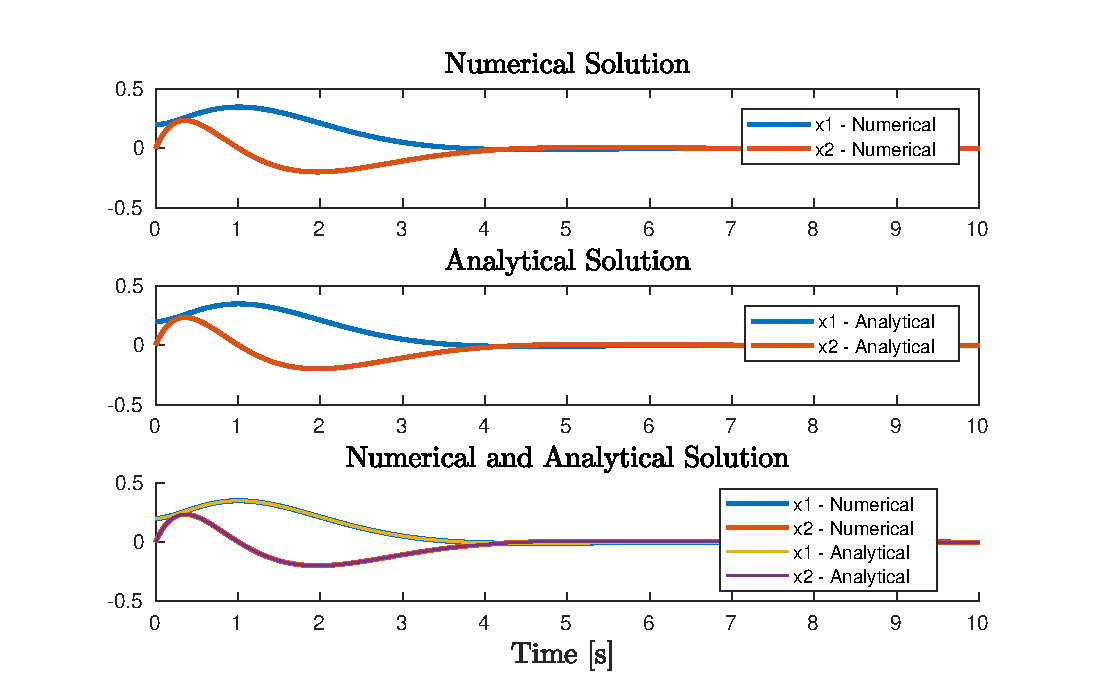
\includegraphics [width=4.5in]{plot.eps}
\end{center}

The next plot shows the difference between three numerical approach to solve the problem and also the analytical response. In this plot shows clearly how important is to choose the right solver.

\includegraphics [width=2\textwidth, angle =90 ]{numerical.eps}


\end{document}
